
%\definecolor{shadecolor}{rgb}{1,0.8,0.3}¹

%\title{Android}
%\author{Ricardo Vaz - PG41097 }
%\date{\today}

%\maketitle

%\tableofcontents

\newpage
\hfill\par
\hfill\par
\centerline{\Huge\textbf Android}\par
\hfill\par
\hfill\par
\section{Arquitetura de Segurança do Android}
\begin{figure}[h!]
\centering
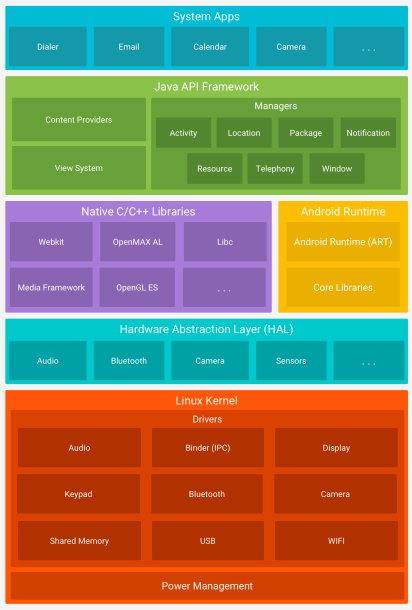
\includegraphics[scale=0.6]{arquiteturaAndroid.png}
\label{fig:arq}
\caption{Arquitetura}
\end{figure}

Android é uma plataforma Open Source baseada em Linux e desenvolvida pelo Google, que serve como um sistema operacional móvel.
Como é possível observar na Figura 1, esta é composta por várias camadas diferentes. Cada camada define interfaces e serviços específicos.


Uma das particularidas das aplicações Android, é o facto destas não terem acesso direto aos recursos de hardware e cada aplicação ser executada na sua própria sandbox, o que permite assim um controlo preciso sobre recursos e aplicativos, por exemplo, quando uma aplicação falha, esta não afetará as restantes aplicações em execução no dispositivo. Outra das particularidades do Android, é que o tempo de execução deste controla o número máximo de recursos do sistema alocados nas aplicações, impedindo, deste modo, que qualquer aplicação monopolize muitos recursos.



\section{Criptografia de dispositivos Android}
Este sistema operativo, suporta criptografia de dispositivo desde da versão 2.3.4 (API nível 10), e que desde então tem passado por grandes mudanças. Por imposição do Google, todos os dispositivos com Android 6.0 (nível 23 da API) ou superior passaram a ter que suportar criptografia de armazenamento, o que em alguns casos veio afetar significativamente o seu desempenho. Criptografia esta que se encontra dividida em três grupos: 
\\
\par \textbf{Full-Disk Encryption} 
Versões 5.0 (nível de API 21) e superiores oferecem suporte à criptografia de disco completo. Esta criptografia usa uma única chave protegida pela senha do dispositivo dos utilizadores para encriptar e desencriptar a partição de dados do utilizador. Este tipo de criptografia, nos tempos atuais, é considerada obsoleta, sendo que, a criptografia baseada em arquivo deve ser, preferencialmente, usada sempre que possível, visto que, a criptografia de disco completo apresenta desvantagens, como não poder receber chamadas ou não ter alarmes operacionais após uma reinicialização se o utilizador não digitar a senha para desbloquear.
\\
\par \textbf{File-Based Encryption}
A versão 7.0 (API nível 24) já suporta criptografia baseada em arquivo. Esta permite que arquivos diferentes sejam encriptados com chaves diferentes, para que possam ser desencriptados independentemente. Fazendo com que os dispositivos que suportam este tipo de criptografia também ofereçam suporte à Inicialização Direta. Esta permite que o dispositivo tenha acesso a recursos como alarmes ou serviços de acessibilidade, mesmo que o utilizador não tenha desbloqueado o dispositivo.
\\
\par \textbf{Adiantum}
A terceira criptografia presente neste sistema operativo, é o Adiantum, em substituição ao AES, que é usado na maioria dos dispositivos Android modernos para criptografia de armazenamento. Na verdade, o AES tornou-se um algoritmo tão amplamente usado que as implementações mais recentes do processador têm um conjunto dedicado de instruções para fornecer operações de encriptação e desencriptação aceleradas por hardware. Porém, nem todos os dispositivos são capazes de usar o AES para criptografia de armazenamento em tempo hábil. 
\par Especialmente dispositivos de última geração com Android Go, pelo facto de usarem processadores low-end, como o ARM Cortex-A7, que não possuem AES acelerado por hardware.
Daí que surgiu o Adiantum, que é uma construção cifrada projetada por Paul Crowley e Eric Biggers no Google para preencher a lacuna desse conjunto de dispositivos que não são capazes de executar o AES pelo menos a 50 MiB/s. 
\par O Adiantum depende apenas de adições, rotações e XORs, essas operações de introdução são suportadas nativamente em todos os processadores. Portanto, os processadores low-end podem encriptar 4 vezes mais rápido e desencriptar 5 vezes mais rápido do que se estivessem usando o AES.
\\
\par Adiantum é uma composição de outras cifras:
\begin{itemize}
    \item NH: Uma função de hash
    \item Poly1305: um código de autenticação de mensagens (MAC)
    \item XChaCha12: Uma cifra de fluxo
    \item AES-256: Uma única invocação do AES
\end{itemize}

\section{Inter-Process Communication (IPC)}
Inter-Process Communication (IPC), ou Comunicação entre Processos, são os recursos que permitem que as aplicações troquem sinais e dados com segurança. Em vez de confiar nas instalações padrão do Linux IPC, o IPC do Android é baseado no Binder, uma implementação personalizada do OpenBinder. Pela segurança transmitida por este, a maioria dos serviços do sistema operativo Android e todos os serviços de comunicação entre pocessos de alto nível dependem do Binder.




\section{Permissões}
Como os aplicativos Android são instalados em uma sandbox e inicialmente não podem aceder a informações do utilizador e componentes do sistema (como a câmera e o microfone), o Android fornece um sistema com um conjunto predefinido de permissões para determinadas tarefas que o aplicativo pode solicitar. 
Por exemplo, para que a aplicação possa usar a câmera do dispositivo, solicitamos a permissão deste modo: \textit{android.permission.CAMERA}

Anteriormente à versão 6.0 (nível 23 da API), todas as permissões solicitadas por uma aplicação eram concedidas aquando a sua instalação. Mas que a partir do nível 23 da API, o utilizador passou a ter que aprovar algumas solicitações de permissão durante a execução do aplicação.


\subsection{Níveis de Proteção}
As permissões do Android são classificadas com base no nível de proteção que oferecem e divididas em quatro categorias diferentes:

\textbf{Normal}: o nível mais baixo de proteção. Ela fornece às aplicações acesso a recursos isolados no nível do aplicativo, com risco mínimo para outras aplicações. Esta é concedida durante a instalação do aplicação e é o nível de proteção padrão.
Exemplo: \textit{android.permission.INTERNET}

\textbf{Perigoso}: esta permissão permite que a aplicação execute ações que possam afetar a privacidade do utilizador ou o funcionamento normal do dispositivo do utilizador. Este nível de permissão pode não ser concedido durante a instalação, pelo que, o utilizador deve decidir se a aplicação deve ter ou não essa permissão.
Exemplo: \textit{android.permission.RECORD\_AUDIO}

\textbf{Assinatura}: esta permissão é concedida somente se a aplicação qua a solicita tiver sido assinada com o mesmo certificado que a aplicação que declarou a permissão. Se a assinatura corresponder, a permissão será concedida automaticamente.
Exemplo: \textit{android.permission.ACCESS\_MOCK\_LOCATION}

\textbf{SystemOrSignature}: esta permissão é concedida apenas a aplicações incorporadas na imagem do sistema ou assinadas com o mesmo certificado com o qual a aplicação que declarou a permissão foi assinada.
\par Exemplo: \textit{android.permission.ACCESS\_DOWNLOAD\_MANAGER}


\subsection{Solicitação de Permissões}
Como visto no início da secção Permissões, as aplicações podem ou não conceder permissões aquando a sua instalação, pelo que as que não o fazem desta forma, são feitas de um outro modo, ou seja, as aplicações podem solicitar permissões para os níveis de proteção Normal, Perigoso e Assinatura, usando para tal, uma tag deste género: \textit{$<$uses-permission /$>$} no manifesto, \textit{AndroidManifest.xml}.



\section{Processo de assinatura e publicação}
Depois de uma aplicação ser desenvolvida com sucesso, o próximo passo é publicá-la e partilhá-la com outras pessoas. No entanto, as aplicaçóes não podem simplesmente ser adicionados a uma loja e partilhadas, sem antes serem assinadas.
A assinatura criptográfica serve como uma marca verificável colocada pelo desenvolvedor da aplicação. Ela identifica o autor da aplicação e garante que esta não tenha sido modificada desde sua distribuição inicial.

\subsection{Processo de assinatura}
Durante o desenvolvimento, as aplicações são assinadas com um certificado gerado automaticamente. Este certificado é inerentemente inseguro e é apenas para depuração. 

A maioria das lojas não aceita este tipo de certificado para publicação, portanto, deve ser criado um certificado com recursos mais seguros. Quando uma aplicação é instalada no dispositivo Android, o Gerenciador de Pacotes garante que ela foi assinado com o certificado incluído no APK correspondente. 

Se a chave pública do certificado corresponder à usada para assinar qualquer outro APK no dispositivo, o novo APK poderá compartilhar um UID (userID) com o APK pré-existente. 
Facilitando, assim, as interações entre aplicações do mesmo fornecedor. Como alternativa, é possível especificar permissões de segurança para o nível de proteção de assinatura, o que restringirá o acesso a aplicações que foram assinadas com a mesma chave.


\subsection{Processo de Publicação}
A distribuição de aplicações para qualquer lugar (no próprio site, qualquer loja etc.) é possível porque o ecossistema do Android está aberto. No entanto, o Google Play é a loja mais conhecida, confiável e popular, e é o próprio Google que a fornece. 

A Amazon Appstore é a loja padrão confiável para dispositivos Kindle. Se os utilizadores quiserem instalar aplicativos de terceiros a partir de uma fonte não confiável, eles deverão permiti-lo explicitamente com as configurações de segurança do dispositivo.

As aplicações podem ser instaladas num dispositivo Android de várias fontes: localmente via USB, via loja de aplicativos oficial do Google (Google Play Store) ou em lojas alternativas.
\\

\par \textit{Nota: Enquanto outros fornecedores podem rever e aprovar aplicações antes de serem realmente publicadas, o Google simplesmente procura assinaturas de malware conhecidas, o que faz com que o tempo entre o início do processo de publicação e a disponibilidade da aplicação ao público seja minimizado.}


\newpage
\section{Android Application Attack Surface}
O aplicativo Android pode estar vulnerável a ataques caso não:
\begin{itemize}
    \item Valide todos os inputs através de uma comunicação IPC ou esquemas de URL
    \item Valide todos os inputs do utilizador nos campos de entrada.
    \item Valide o conteúdo carregado dentro de uma página Web.
    \item Comunique de forma segura com os servidores que prestam serviços ou seja suscetivel a ataques man-in-the-middle.
    \item Armazene com segurança todos os dados locais ou carregue dados não confiáveis do armazenamento.
    \item Tenha proteção contra ambientes comprometidos, reempacotamento ou outros ataques
\end{itemize}



\section{TESTES DE SEGURANÇA EM APLICAÇÕES}

\subsection{Data Storage on Android}
Os dados públicos devem estar disponíveis para todos, mas os dados confidenciais e privados devem ser protegidos ou, melhor ainda, mantidos fora do armazenamento do dispositivo.

Para além de proteger dados confidenciais, é necessário garantir que os dados lidos de qualquer fonte de armazenamento sejam validados e possivelmente limpos. Esta validação geralmente serve para garantir que os dados apresentados sejam do tipo solicitado, mas com o uso de HMAC's é possível validar a correção dos dados.


\subsubsection{Testar o armazenamento local para dados confidenciais (MSTG-STORAGE-1 e MSTG-STORAGE-2)}\par
\hfill\par
\hfill\par
Por norma, deve-se armazenar o mínimo possível de dados sensíveis no armazenamento local permanentemente. No entanto, algum tipo de dado do utilizador deve ser armazenado. Por exemplo, pedir ao utilizador que insira uma senha muito complexa de todas as vezes que a aplicação inicie não é uma boa idéia em termos de usabilidade. Deste modo, as aplicações devem armazenar em cache algum tipo de token de autenticação para evitar isso.
\\
\\
Os dados confidenciais ficam vulneráveis quando não estão adequadamente protegidos pela aplicação que os armazena persistentemente, o que pode levar, à divulgação de informações confidenciais. Em geral, um atacante pode identificar essas informações e usá-las em ataques adicionais, como engenharia social, sequestro de contas (se as informações da sessão ou um token de autenticação tiverem sido divulgados), ou ainda, a recolha de informações de aplicações que possuem uma opção de pagamento.
\\
\\
\\
\\
\\
\\
Os dados podem ser armazenados persistentemente de várias maneiras, entre as quais:
\begin{itemize}
    \item Preferências Compartilhadas
    \item Bases de dados SQLite
    \item Bases de dados Firebase
    \item Armazenamento interno
    \item Armazenamento externo
\end{itemize}


\textbf{Preferências Compartilhadas}
\par A API SharedPreferences é frequentemente usada para salvar permanentemente pequenas coleções de pares de valores-chave. Os dados armazenados em um objeto SharedPreferences são gravados em um arquivo XML de texto sem formatação. 
\par O objeto SharedPreferences pode ser declarado legível (acessível a todos as aplicações) ou privado. A API SharedPreferences geralmente pode levar à exposição de dados confidenciais.
\\
\par \textbf{Bases de dados SQLite}
\begin{itemize}
    \item \textbf{Bases de dados SQLite (não encriptadas)} - SQLite é um mecanismo de banco de dados SQL que armazena dados em arquivos .db. O Android SDK possui suporte interno para bancos de dados SQLite. O pacote principal usado para gerenciar os bancos de dados é android.database.sqlite. \par
\hfill\par
\item \textbf{Bases de dados SQLite (encriptadas)} - Se as bases de dados SQLite encriptadas forem usadas, a senha estará codificada na fonte, armazenada em preferências compartilhadas ou oculta noutro lugar no código ou no sistema de arquivos. 
\par As formas seguras de recuperar a chave incluem:
    \begin{itemize}
        \item Solicitando ao utilizador que decodifique a base de dados com um PIN ou senha assim que a aplicação for aberta (senhas e PINs fracos são vulneráveis a ataques de força bruta)\par
        \hfill\par
        \item Armazenando a chave no servidor e permitindo que ela seja acessada apenas a partir de um serviço da Web (para que a aplicação possa ser usada apenas quando o dispositivo estiver online)
    \end{itemize}
\end{itemize}

\hfill\par
\textbf{Bancos de dados Firebase}\par
\hfill\par
\par O Firebase é uma plataforma de desenvolvimento que pode ser aproveitada para armazenar e sincronizar dados de uma aplicção com um banco de dados hospedado na nuvem NoSQL. Os dados são armazenados como JSON e são sincronizados em tempo real com todos os clientes conectados e também permanecem disponíveis mesmo quando o aplicativo fica offline.
\\
\par \textbf{Armazenamento interno}
\par É possível salvar arquivos no armazenamento interno do dispositivo. Os arquivos salvos no armazenamento interno são containers por padrão e não podem ser acessedidos por outras aplicações no dispositivo, e quando o utilizador desinstala a aplicação, esses arquivos são removidos.
\\
\par \textbf{Armazenamento externo}
\par Outra das possibilidades, é o armazenamento externo compartilhado. Esse armazenamento pode ser removível (como um cartão SD) ou interno (não removível). Os arquivos salvos no armazenamento externo são legíveis. O utilizador pode modificá-los quando o armazenamento USB estiver ativado.



\subsubsection{Determinar se dados sensíveis são enviados a terceiros (MSTG-STORAGE-4)}\par
\hfill\par
\hfill\par
\par A possibilidade de incorporar serviços de terceiros nas aplicações, é que este tipo de serviços podem ter implementados serviços de rastreamento, monitorização do comportamento do utilizador, venda de anúncios em banner, entre outros.
\par Pelo que a desvantagem, neste tipo de serviços é a falta de visibilidade, ou seja, não sabermos exatamente qual o código que executam. Desta forma, deve garantir-se que apenas sejam enviadas as informações não sensíveis necessárias.


\subsubsection{Procurar dados sensíveis na cache do teclado (MSTG-STORAGE-5)}\par
\hfill\par
\hfill\par
\par A inserção de dados por parte dos utilizadores, é algo que pode ser comprometer informações confidenciais. Ou seja, quando os utilizadores inserem informação nos campos de entrada, o software sugere dados automaticamente, o que em parte pode ser muito útil para aplicações de mensagens, mas, em contrapartida, a cache do teclado pode divulgar informações confidenciais quando o utilizador seleciona um campo de entrada que aceita esse tipo de informação, pelo que se torna necessário limpar a cache do teclado de vez enquando.



\subsubsection{Verificar a divulgação confidencial de dados por meio da interface do utilizador (MSTG-STORAGE-7)}\par
\hfill\par
\hfill\par
\par São enumeras as aplicações que exigem que os utilizadores insiram vários tipos de dados para, por exemplo, registrar uma conta ou efetuar um pagamento, entre outros. 
\par Este tipo de aplicaçóes requerem alguns cuidados, visto que ocorre a exposição de dados confidenciais, pelo que, é imperativo que estes não sejam mostrados em texto limpo na interface após inseridos. Os dados dados confidenciais devem então ser mascarados, através de asteriscos ou pontos em vez de texto não encriptado.



\subsection{Android Cryptographic APIs}\par
\hfill\par
\subsubsection{Testando a configuração de algoritmos padrão criptográficos (MSTG-CRYPTO-2, MSTG-CRYPTO-3 e MSTG-CRYPTO-4)}\par
\hfill\par
\hfill\par
\par As APIs de criptografia do Android são baseadas em Java Cryptography Architecture (JCA). Esta separa as interfaces e a implementação, o que possibilita incluir vários provedores de segurança que podem implementar conjuntos de algoritmos criptográficos.
\par A maioria das interfaces e classes JCA são definidas nos pacotes java.security.* e javax.crypto.*. Para além disso, existem ainda pacotes específicos para Android, android.security.* e android.security.keystore.*.

\par A lista de provedores incluídos no Android varia consoante a versão do Android e as compilações específicas do Original Equipment Manufacturer (OEM). Atualmente, algumas implementações de provedor, em versões mais antigas são mais inseguras/vulneráveis. Portanto, as aplicações Android não devem apenas escolher os algoritmos corretos e fornecer uma boa configuração, em alguns casos, também devem prestar atenção à força das implementações nos provedores legados.



\subsubsection{Teste do manutenção de chaves (MSTG-STORAGE-1, MSTG-CRYPTO-1 e MSTG-CRYPTO-5)}\par
\hfill\par
\hfill\par
\par Quando o assunto são chaves criptográficas, deve ter se especial atenção, visto existirem tanto maneiras seguras como inseguras para o seu armazenamento. 
\par A maneira mais segura de manusear conteúdos importantes, simplesmente é nunca armazená-los no dispositivo, ou seja, o que significa que o utilizador deve ser solicitado a inserir uma senha sempre que a aplicação precisar de executar uma operação criptográfica, o que do do ponto de vista da experiência do utilizador torna-se inpensável. A razão disto é que o conteúdo principal estaja disponível apenas numa matriz na memória enquanto estiver a ser usado, e quando a chave não estiver a ser necessária, a matriz pode ser zerada, o que minimiza a janela de ataque. Nenhum conteúdo importante afeta o sistema de arquivos e nenhuma senha é armazenada. 

\par No entanto, deve-se ter em consideração que algumas cifras não limpam adequadamente as suas matrizes de bytes. Por exemplo, a codificação AES no BouncyCastle nem sempre limpa a sua última chave de trabalho. De seguida, as chaves baseadas no BigInteger (por exemplo, chaves privadas) não podem ser removidas do heap nem zeradas. E claro, deve-se tomar especial atenção ao tentar zerar a chave. 



\subsubsection{Testar a geração de números aleatórios (MSTG-CRYPTO-6)}\par
\hfill\par
\hfill\par
\par A criptografia requer geração segura de números pseudo-aleatórios (PRNG).
\par As classes Java padrão não fornecem aleatoriedade suficiente e, de fato, podem permitir que um atacante adivinhe o próximo valor que será gerado e use esse palpite para representar outro utilizador ou aceder a informações confidenciais.

\par Para tal, deve ser usado o SecureRandom, o qual deve ser instanciado por meio do construtor padrão sem argumentos. Outros construtores são para usos mais avançados e, se usados incorretamente, podem levar à diminuição da aleatoriedade e segurança. O provedor PRNG que apoia o SecureRandom usa o arquivo de dispositivo \textit{/dev/urandom} como fonte de aleatoriedade por padrão.






\subsection{Local Authentication on Android}
\par Durante a autenticação local, uma aplicação autentica um utilizador verificando con credenciais guardadas localmente no dispositivo (PIN, password, carateristicas biometricas), que são verificados por referência a dados locais. Este processo é realizado para que os utilizadores possam retomar mais convenientemente uma sessão existente com um serviço remoto ou como um meio de autenticação avançada para proteger algumas funções críticas.



\subsubsection{Testar credenciais de confirmação (MSTG-AUTH-1 e MSTG-STORAGE-11)}\par
\hfill\par
\hfill\par
\par O fluxo de confirmação da credencial está disponível desde da versão 6.0 e é usada para garantir que os utilizadores não precisem de inserir senhas específicas da aplicação junto com a proteção da tela de bloqueio. 

\par Em vez disso, se um utilizador que fez login no dispositivo recentemente, as suas credenciais de confirmação podem ser usadas para desbloquear conteúdos criptográficos na AndroidKeystore. Ou seja, se o utilizador desbloqueou o dispositivo dentro dos limites de tempo definidos (setUserAuthenticationValidityDurationSeconds), caso contrário, o dispositivo precisará de ser desbloqueado novamente.





%-------------------------------------------------------------------------------------------------------%
\subsection{Android Network APIs}

\subsubsection{Testar a verificação de identificação de terminal (MSTG-NETWORK-3)}\par
\hfill\par
\hfill\par
\par Uma das medidas de segurança para transporte de informação confidencial pela rede é o o uso do TLS. Porém, a comunicação encriptada entre uma aplicação móvel e a sua API de back-end não é trivial. 

\par Por norma, as soluções mais simples, mas menos seguras, como por exemplo, aquelas que aceitam qualquer certificado, para facilitar o processo de desenvolvimento, são soluções fracas que entram na versão de produção, e que acabam por expor os utilizadores a ataques man-in-the-middle.

\par Daí que surgem duas medidas essencias, nomeadamente:
\begin{itemize}
    \item Verificar se um certificado provém de uma fonte confiável, ou seja, uma CA (Autoridade de Certificação) confiável.
    \item Determinar se o servidor do nó da extremidade apresenta o certificado correto.
\end{itemize}




\subsubsection{Testando armazenamentos de certificados personalizados e fixação de certificados (MSTG-NETWORK-4)}\par
\hfill\par
\hfill\par
\par O processo de armazenamento de certificados e fixação de certificados é algo a que se deve prestar especial atenção, pois a aceitação de qualquer certificado assinado pode ser um processo compremetedor, ou seja, apenas deve ser feita a aceitação de certificados assinados por autoridades de certificação de confiança.

\par A fixação de certificado é o processo de associar o servidor back-end a um certificado X.509 ou chave pública específica, em vez de aceitar qualquer certificado assinado por uma autoridade de certificação confiável. Após armazenar o certificado ou a chave pública do servidor, a aplicação móvel conectar-se-á, posteriormente, apenas ao servidor conhecido. 

\par Em suma, retirar a confiança de autoridades de certificação externas reduz a superfície de ataque, visto existirem enumeros casos de autoridades de certificação que foram comprometidas ou enganadas na emissão de certificados por impostores.

\par O certificado pode ser fixado e codificado na aplicação ou recuperado no momento em que esta se conecta ao back-end. Neste último caso, o certificado é associado ao fixado ao host, e aquando o host é visto pela primeira vez. O que torna esta alternativa menos segura, porque os atacantes que interceptem a conexão inicial podem injetar os seus próprios certificados.






\subsection{Android Platform APIs}
\subsubsection{Testar permissões de aplicativos (MSTG-PLATFORM-1)}\par
\hfill\par
\hfill\par
\par O Android atribui uma identidade distinta do sistema a todos as aplicações instaladas, e como cada aplicação opera numa área restrita de processo, as aplicações devem solicitar explicitamente o acesso a recursos e dados que estão fora da área restrita. 

\par Para tal, elas solicitam este acesso declarando as permissões necessárias para usar os dados e recursos do sistema, e dependendo do quão sensíveis ou críticos sejam os dados ou os recursos, o próprio sistema Android concederá a permissão automaticamente ou, então, solicitará que o utilizador aprove a solicitação.

Como já referido anteriormente na secção "Permissões", estas são classificadas em quatro categorias diferentes com base no nível de proteção que oferecem:

\begin{itemize}
    \item Normal: concede às aplicações acesso a recursos isolados no nível da aplicação com risco mínimo para outras aplicações. Exemplo: android.permission.INTERNET

    \item Perigoso: geralmente concede à aplicação controlo sobre os dados do utilizador ou sobre o dispositivo de uma maneira que pode afetar o utilizador. 
    Exemplo: android.permission.RECORD\_AUDIO

    \item Assinatura: esta permissão é concedida apenas se a aplicação solicitante tiver sido assinada com o mesmo certificado usado para assinar a aplicação que declarou a permissão. 
    Exemplo: android.permission.ACCESS\_MOCK\_LOCATION

    \item SystemOrSignature: esta permissão é concedida apenas a aplicações incorporadas na imagem do sistema ou assinadas com o mesmo certificado usado para assinar a aplicação que declarou a permissão. 
    \par Exemplo: android.permission.ACCESS\_DOWNLOAD\_MANAGER
\end{itemize}



\subsubsection{Testar exposição sensível à funcionalidade através do IPC (MSTG-PLATFORM-4)}\par
\hfill\par
\hfill\par
Durante a implementação de uma aplicação móvel, os desenvolvedores podem usar técnicas tradicionais para IPC (como ficheiros ou sockets partilhadas), as funcionalidades do IPC para aplicações devem ser usadas visto serem muito mais seguras para não haver comprometimento de dados.


\par A funcionalidade do sistema IPC oferecida pelas plataformas de aplicações móveis deve ser usada, por ser muito mais maduro que as técnicas tradicionais. O uso de mecanismos IPC sem segurança pode fazer com que a aplicação vaze ou exponha dados confidenciais.

\par Mecanismos IPC do Android, como Binders, Services, Bound Services, AIDL (Android Interface Definition Language), Intents, ou Content Providers, são mecanismos que podem levar à exposição de dados confidenciais.



